% !TeX program = xelatex
% !TeX encoding = UTF-8
% !TeX TXS-program:compile = txs:///xelatex | txs:///xelatex
\documentclass[aspectratio=169, table, 12pt]{beamer}
% Preamble bersama seluruh slide mata kuliah ini.
% Dipanggil dari slides/sessionXX/sessionXX.tex tepat sesudah baris
% \documentclass[aspectratio=169, table, 12pt]{beamer}
% Paket tambahan yang hanya dibutuhkan satu sesi ditulis di berkas sesi itu.

\usepackage{colortbl}
\usepackage{xcolor}
\usepackage{listings}
\usepackage{tabularx}
\usepackage{booktabs}
\usepackage{tikz}
\usepackage{pgfplots}
\pgfplotsset{compat=1.18}
\usetikzlibrary{arrows.meta, positioning, calc, fit, shapes.geometric,
	shapes.multipart, backgrounds, matrix, chains, trees}

\makeatletter
\def\input@path{{../theme/}}
\makeatother
\graphicspath{{../theme/}{../../figures/}}
\usetheme{Pradita}

\definecolor{praditagreen}{RGB}{37, 113, 71}

% Tema membuat garis tabel berwarna putih. Dikembalikan agar tabel terbaca.
\arrayrulecolor{black}
\setlength{\arrayrulewidth}{0.5pt}

\lstdefinelanguage{yaml}{
	basicstyle=\ttfamily\scriptsize,
	keywordstyle=\color{blue}\bfseries,
	commentstyle=\color{gray}\itshape,
	stringstyle=\color{red},
	showstringspaces=false,
	breaklines=true,
	frame=lines,
	numbers=none,
	backgroundcolor=\color{lightgray!10},
	tabsize=2,
	morecomment=[l]{\#}
}

\lstdefinelanguage{json}{
	basicstyle=\ttfamily\scriptsize,
	stringstyle=\color{red},
	commentstyle=\color{gray},
	breaklines=true,
	showstringspaces=false,
	tabsize=2,
	numbers=none,
	frame=lines,
	backgroundcolor=\color{lightgray!10},
	string=[s]{"}{"}
}

\lstdefinelanguage{bash}{
	keywords={},
	basicstyle=\ttfamily\scriptsize,
	ndkeywords={docker, kubectl, helm, curl, git, terraform},
	ndkeywordstyle=\color{purple}\bfseries,
	sensitive=true,
	commentstyle=\color{gray},
	numbers=none,
	breaklines=true,
	frame=lines,
	backgroundcolor=\color{lightgray!10},
	tabsize=2,
	comment=[l]{\#},
	showstringspaces=false
}

\lstdefinelanguage{http}{
	keywords={GET, POST, PUT, PATCH, DELETE, HEAD, OPTIONS, HTTP},
	basicstyle=\ttfamily\scriptsize,
	keywordstyle=\color{blue}\bfseries,
	sensitive=true,
	numbers=none,
	breaklines=true,
	frame=lines,
	backgroundcolor=\color{lightgray!10},
	tabsize=2,
	showstringspaces=false
}

\subtitle{IT40613 · Digital Platform \& API Economy}
\author{\textbf{Alfa Yohannis}}


\title{\Huge Model Bisnis Platform\\ \vspace{10pt} dan Efek Jaringan}
\date{Pertemuan 02}

\begin{document}
\frame{\titlepage}

\begin{frame}
  \frametitle{Isi Pertemuan}
  \vspace{14pt}
  \begin{columns}[t]
    \column{0.5\textwidth}
    {\small\tableofcontents[sections={1-3}]}

    \column{0.5\textwidth}
    {\small\tableofcontents[sections={4-5}]}
  \end{columns}
\end{frame}

\begin{frame}{\hfill}
  \centering
  \Huge{\textbf{Klinik menunggu pasien,\\pasien menunggu klinik.\\Sisi mana yang\\datang lebih dulu?}}
\end{frame}

\section{Sisi Pasar dan Interaksi Inti}

\begin{frame}{\hfill}
  \centering
  \Huge{\textbf{Sisi Pasar dan\\Interaksi Inti}}
\end{frame}

\begin{frame}{{\Large Tujuan Pembelajaran}}
  \vspace{10pt}
  \begin{itemize}
    \item Mengidentifikasi sisi pasar, interaksi inti, dan nilai bagi tiap sisi pada sebuah platform.
    \item Membedakan efek jaringan sisi sama dan lintas sisi, baik yang positif maupun yang negatif.
    \item Menganalisis strategi mengatasi masalah ayam dan telur (\textit{chicken-and-egg problem}) saat platform diluncurkan.
  \end{itemize}
\end{frame}

\begin{frame}{{\Large Persoalan Medikara Health}}
  \vspace{10pt}
  \begin{itemize}
    \item Direksi sepakat membuka Medikara+ bagi klinik mitra dan perusahaan asuransi.
    \item Klinik mau bergabung bila pasiennya banyak. Pasien mau memakai aplikasi bila pilihan dokternya banyak.
    \item Tim pemasaran mengusulkan layanan gratis bagi pasien. Tim keuangan meminta klinik membayar langganan.
    \item Perusahaan asuransi bertanya apa untungnya bagi mereka.
    \item Pertanyaan ini adalah pertanyaan model bisnis platform, bukan pertanyaan tim teknologi.
  \end{itemize}
\end{frame}

\begin{frame}{{\Large Dua Syarat Platform Multi-Sisi}}
  \begin{itemize}
    \item Hagiu dan Wright: nilai diciptakan terutama lewat interaksi langsung antara dua jenis pelanggan atau lebih.
    \item Interaksi langsung: kedua sisi memegang kendali atas syarat utama, misalnya harga dan isi layanan.
    \item Afiliasi: setiap sisi dengan sadar bergabung, misalnya mendaftar atau membayar keanggotaan.
    \item Dua jenis pelanggan: pasar dua sisi. Tiga atau lebih: pasar multi-sisi.
    \item Cusumano dkk.: platform transaksi menjadi perantara, platform inovasi menjadi fondasi pihak ketiga, keduanya sekaligus disebut hibrida.
  \end{itemize}
  \vspace{2pt}
  {\footnotesize Analogi: pemilik toko kelontong menentukan harga sendiri. Pengelola pasar hanya menyewakan lapak.\par}
\end{frame}

\begin{frame}{{\Large Pengecer, Pipeline, dan Platform Multi-Sisi}}
  \footnotesize
  \begin{tabularx}{\textwidth}{>{\raggedright\arraybackslash}p{2.4cm}
      >{\raggedright\arraybackslash}X
      >{\raggedright\arraybackslash}X}
    \hline
    \textbf{Model} & \textbf{Penentu harga dan syarat} & \textbf{Contoh layanan kesehatan} \\ \hline
    Pengecer & Pengecer sendiri; pemasok tidak berhubungan dengan pembeli & Apotek yang membeli obat dari distributor lalu menjualnya \\ \hline
    \textit{Pipeline} & Perusahaan; tenaga kerja tidak berafiliasi dengan pelanggan & Rumah sakit yang menggaji dokter dan menetapkan tarif \\ \hline
    Platform multi-sisi & Kedua sisi; keduanya mendaftar ke platform & Aplikasi tempat dokter menetapkan jadwal dan tarif sendiri \\ \hline
  \end{tabularx}

  \vspace{6pt}
  Rumah sakit Medikara di Bekasi menetapkan tarif spesialis Rp250.000 dan menagih atas nama rumah sakit: \textit{pipeline}. Misalkan 40 klinik pratama mitra menetapkan tarif sendiri, Rp90.000 sampai Rp150.000 per konsultasi: bagian ini bekerja sebagai platform.
\end{frame}

\begin{frame}{{\Large Calon Sisi Pasar Medikara+}}
  \centering
  \resizebox{!}{0.62\textheight}{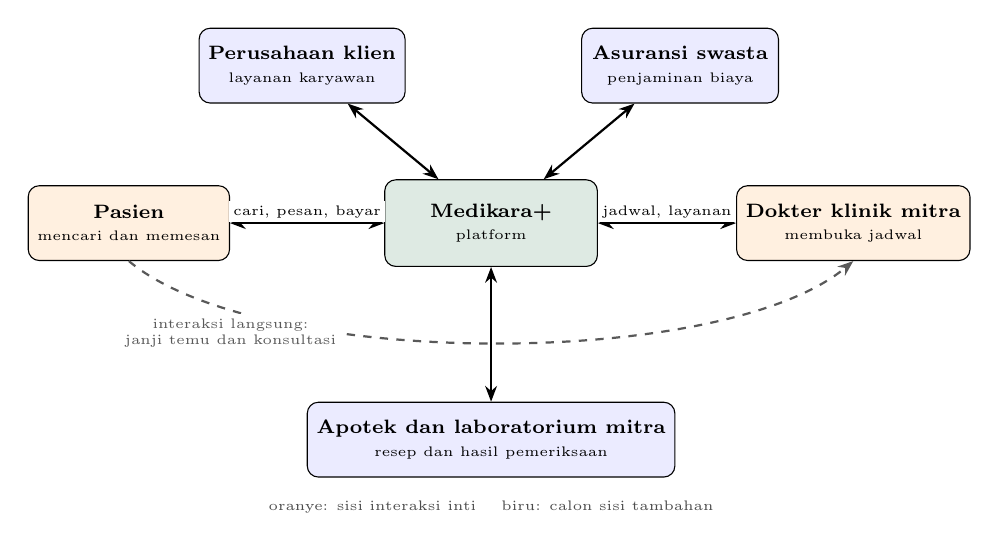
\begin{tikzpicture}[
  font=\scriptsize,
  kotak/.style={draw, rounded corners, minimum height=0.95cm, minimum width=2.5cm,
                align=center, font=\scriptsize\bfseries},
  panah/.style={-{Stealth[length=2mm]}, thick},
  duaarah/.style={{Stealth[length=2mm]}-{Stealth[length=2mm]}, thick},
  ket/.style={font=\tiny, align=center, fill=white, inner sep=1.5pt}
]
  \node[kotak, fill=praditagreen!15, minimum width=2.7cm, minimum height=1.1cm] (inti)
    at (0,0) {Medikara+\\{\tiny\mdseries platform}};

  \node[kotak, fill=orange!12] (pasien) at (-4.6,0)
    {Pasien\\{\tiny\mdseries mencari dan memesan}};
  \node[kotak, fill=orange!12] (dokter) at (4.6,0)
    {Dokter klinik mitra\\{\tiny\mdseries membuka jadwal}};
  \node[kotak, fill=blue!8] (perusahaan) at (-2.4,2.0)
    {Perusahaan klien\\{\tiny\mdseries layanan karyawan}};
  \node[kotak, fill=blue!8] (asuransi) at (2.4,2.0)
    {Asuransi swasta\\{\tiny\mdseries penjaminan biaya}};
  \node[kotak, fill=blue!8, minimum width=3.4cm] (apotek) at (0,-2.75)
    {Apotek dan laboratorium mitra\\{\tiny\mdseries resep dan hasil pemeriksaan}};

  \draw[duaarah] (pasien) -- node[ket, above] {cari, pesan, bayar} (inti);
  \draw[duaarah] (dokter) -- node[ket, above] {jadwal, layanan} (inti);
  \draw[duaarah] (perusahaan) -- (inti);
  \draw[duaarah] (asuransi) -- (inti);
  \draw[duaarah] (apotek) -- (inti);

  % Busur dilandaikan agar tidak menyentuh kotak apotek, dan labelnya di luar panah tengah.
  \draw[panah, dashed, gray!70!black] (pasien.south) to[out=-40, in=-140, looseness=0.6]
    node[ket, below, pos=0.2, xshift=-4pt] {interaksi langsung:\\janji temu dan konsultasi}
    (dokter.south);

  \node[font=\tiny, anchor=north, align=center, text=gray!60!black] at (0,-3.4)
    {oranye: sisi interaksi inti \quad biru: calon sisi tambahan};
\end{tikzpicture}
}

  \vspace{2pt}
  {\footnotesize Tahap awal adalah platform transaksi. Platform inovasi baru terbentuk bila Medikara membuka \textit{Application Programming Interface} (API).\par}
\end{frame}

\begin{frame}{{\Large Siapa Sisi Pasar Medikara+?}}
  \begin{block}{Kasus Medikara Health}
    \small
    \begin{itemize}
      \item Pasien dan dokter klinik mitra memenuhi kedua syarat dan membentuk interaksi inti.
      \item Dokter internal berada di wilayah abu-abu: tarif tatap muka ditetapkan Medikara, telekonsultasi sukarela.
      \item Asuransi swasta, perusahaan klien, serta apotek dan laboratorium mitra ditunda sampai interaksi inti berjalan.
      \item Badan Penyelenggara Jaminan Sosial (BPJS) Kesehatan bukan sisi pasar: tarif dan aturan klaimnya tidak dirundingkan lewat Medikara+.
    \end{itemize}
  \end{block}
\end{frame}

\begin{frame}{{\Large Interaksi Inti: Partisipan, Unit Nilai, Filter}}
  \begin{itemize}
    \item Interaksi inti (\textit{core interaction}) adalah pertukaran nilai terpenting pada platform.
    \item Partisipan: produsen yang menciptakan nilai dan konsumen yang memakainya.
    \item Unit nilai (\textit{value unit}): informasi dari produsen, misalnya slot jadwal dokter.
    \item Filter: aturan atau algoritma yang menentukan unit nilai mana yang sampai ke konsumen.
    \item Tiga fungsi platform: menarik (\textit{pull}), memudahkan (\textit{facilitate}), dan mencocokkan (\textit{match}).
  \end{itemize}
  \vspace{2pt}
  {\footnotesize Analogi: papan lowongan di bursa kerja kampus. Petugas memilah lowongan menurut jurusan.\par}
\end{frame}

\begin{frame}{{\Large Interaksi Inti Pemesanan Janji Temu}}
  \centering
  \resizebox{0.86\textwidth}{!}{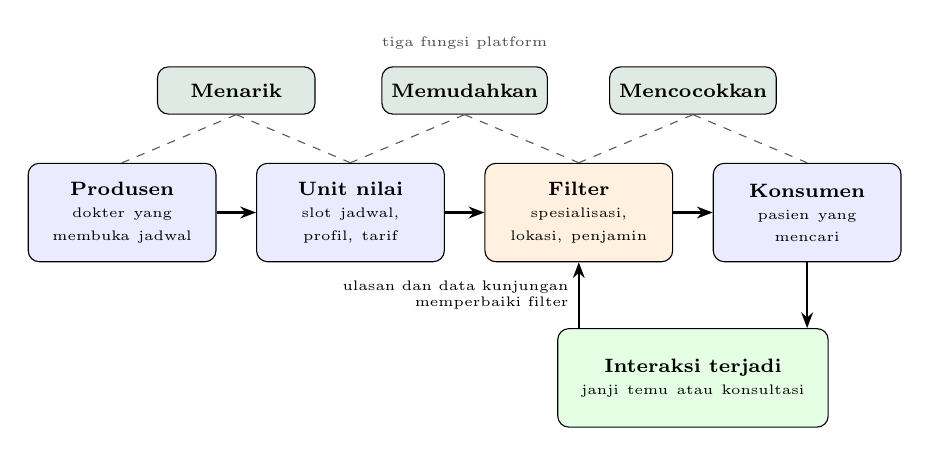
\begin{tikzpicture}[
  font=\scriptsize,
  kotak/.style={draw, rounded corners, minimum height=1.25cm, text width=2.15cm,
                align=center, font=\scriptsize\bfseries},
  fungsi/.style={draw, rounded corners, minimum height=0.6cm, minimum width=2.0cm,
                 align=center, fill=praditagreen!15, font=\scriptsize\bfseries},
  panah/.style={-{Stealth[length=2mm]}, thick},
  garis/.style={dashed, gray!70!black}
]
  \node[kotak, fill=blue!8] (produsen) at (0,0)
    {Produsen\\{\tiny\mdseries dokter yang membuka jadwal}};
  \node[kotak, fill=blue!8] (unit) at (2.9,0)
    {Unit nilai\\{\tiny\mdseries slot jadwal, profil, tarif}};
  \node[kotak, fill=orange!12] (filter) at (5.8,0)
    {Filter\\{\tiny\mdseries spesialisasi, lokasi, penjamin}};
  \node[kotak, fill=blue!8] (konsumen) at (8.7,0)
    {Konsumen\\{\tiny\mdseries pasien yang mencari}};
  \node[kotak, fill=green!10, text width=3.2cm] (interaksi) at (7.25,-2.1)
    {Interaksi terjadi\\{\tiny\mdseries janji temu atau konsultasi}};

  \draw[panah] (produsen) -- (unit);
  \draw[panah] (unit) -- (filter);
  \draw[panah] (filter) -- (konsumen);
  % Kedua panah tegak lurus terhadap kotak interaksi, supaya tidak masuk ke dalam kotak.
  \draw[panah] (konsumen.south) -- (konsumen.south |- interaksi.north);
  \draw[panah] (filter.south |- interaksi.north) --
    node[font=\tiny, align=right, midway, left]
    {ulasan dan data kunjungan\\memperbaiki filter} (filter.south);

  \node[fungsi] (tarik) at (1.45,1.55) {Menarik};
  \node[fungsi] (mudah) at (4.35,1.55) {Memudahkan};
  \node[fungsi] (cocok) at (7.25,1.55) {Mencocokkan};
  \draw[garis] (tarik.south) -- (produsen.north);
  \draw[garis] (tarik.south) -- (unit.north);
  \draw[garis] (mudah.south) -- (unit.north);
  \draw[garis] (mudah.south) -- (filter.north);
  \draw[garis] (cocok.south) -- (filter.north);
  \draw[garis] (cocok.south) -- (konsumen.north);
  \node[font=\tiny, text=gray!60!black, anchor=south] at (4.35,1.95)
    {tiga fungsi platform};
\end{tikzpicture}
}

  \vspace{4pt}
  {\footnotesize Filter ditekankan karena di sanalah platform menambah nilai paling besar.\par}
\end{frame}

\begin{frame}{{\Large Peran Filter: Dua Contoh}}
  \vspace{6pt}
  \begin{itemize}
    \item Misalkan Medikara+ menampilkan 1.400 slot jadwal per hari dari sekitar 640 dokter.
    \item Tanpa filter, seorang ibu di Depok menggulir ratusan slot yang tidak relevan.
    \item Dengan filter spesialisasi, radius 10 km, dan penjamin, pilihannya menyusut menjadi 18 slot.
    \item Misalkan filter hanya mengurutkan menurut jumlah ulasan: jadwal dokter lama penuh sampai tiga minggu.
    \item Dokter baru hampir tidak terlihat, lalu pergi. Platform kehilangan produsen yang dibutuhkan.
  \end{itemize}
\end{frame}

\begin{frame}{{\Large Memilih Interaksi Inti Medikara+}}
  \begin{block}{Kasus Medikara Health}
    \small
    \begin{itemize}
      \item Bab 1: sekitar 28.000 janji temu per bulan lewat Medikara+, yaitu 336.000 per tahun.
      \item Telekonsultasi: 6.000 pasien aktif per bulan, rata-rata 0,3 konsultasi, yaitu 21.600 per tahun.
      \item Janji temu sekitar lima belas kali lebih besar, sehingga dipilih sebagai interaksi inti.
      \item Slot jadwal disimpan di lima Sistem Informasi Manajemen Rumah Sakit (SIMRS) dengan versi berbeda.
      \item Slot diperbarui setiap lima menit. Misalkan 1\% pemesanan, atau 280 per bulan, bentrok dengan pendaftaran di loket.
    \end{itemize}
  \end{block}
\end{frame}

\section{Efek Jaringan}

\begin{frame}{\hfill}
  \centering
  \Huge{\textbf{Efek Jaringan}}
\end{frame}

\begin{frame}{{\Large Apa Itu Efek Jaringan}}
  \begin{itemize}
    \item Efek jaringan (\textit{network effect}): nilai platform bagi seorang pengguna berubah karena jumlah pengguna lain.
    \item Efek sisi sama, disebut juga efek langsung, terjadi di antara pengguna pada sisi yang sama.
    \item Efek lintas sisi, disebut juga efek tidak langsung, terjadi di antara dua sisi.
    \item Keduanya dapat positif atau negatif.
    \item Eisenmann dan rekan: efek lintas sisi biasanya positif, efek sisi sama sering negatif.
  \end{itemize}
  \vspace{2pt}
  {\footnotesize Analogi: pasar malam. Pedagang menarik pengunjung, tetapi pengunjung yang terlalu padat membuat orang sulit berjalan.\par}
\end{frame}

\begin{frame}{{\Large Peta Efek Jaringan Medikara+}}
  \centering
  \resizebox{0.92\textwidth}{!}{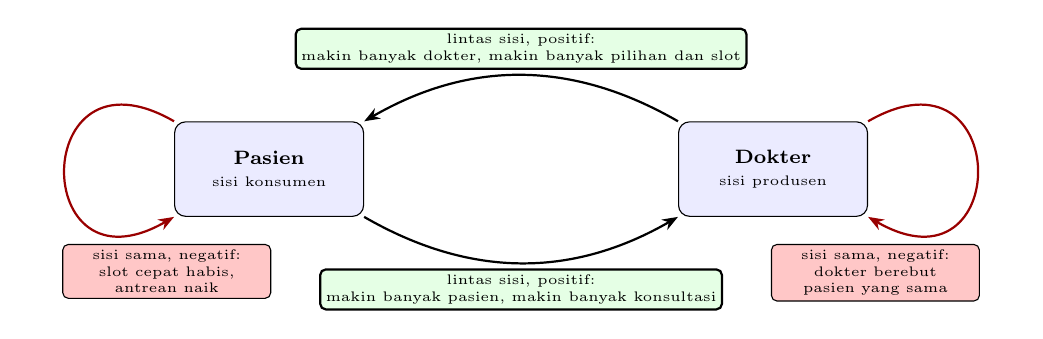
\begin{tikzpicture}[
  font=\scriptsize,
  kotak/.style={draw, rounded corners, minimum height=1.2cm, minimum width=2.4cm,
                align=center, font=\scriptsize\bfseries, fill=blue!8},
  panah/.style={-{Stealth[length=2mm]}, thick},
  positif/.style={draw, rounded corners=2pt, fill=green!10, font=\tiny,
                  align=center, inner sep=2pt},
  negatif/.style={draw, rounded corners=2pt, fill=red!22, font=\tiny,
                  align=center, inner sep=2pt}
]
  \node[kotak] (pasien) at (0,0) {Pasien\\{\tiny\mdseries sisi konsumen}};
  \node[kotak] (dokter) at (6.4,0) {Dokter\\{\tiny\mdseries sisi produsen}};

  \draw[panah] (dokter.north west) to[out=150, in=30]
    node[positif, above, yshift=2pt] {lintas sisi, positif:\\
      makin banyak dokter, makin banyak pilihan dan slot}
    (pasien.north east);
  \draw[panah] (pasien.south east) to[out=-30, in=-150]
    node[positif, below, yshift=-2pt] {lintas sisi, positif:\\
      makin banyak pasien, makin banyak konsultasi}
    (dokter.south west);

  \draw[panah, red!60!black] (pasien.north west) to[out=150, in=210, looseness=4.5]
    (pasien.south west);
  \node[negatif, anchor=north, text width=2.5cm] at (-1.3,-0.95)
    {sisi sama, negatif:\\slot cepat habis, antrean naik};

  \draw[panah, red!60!black] (dokter.north east) to[out=30, in=-30, looseness=4.5]
    (dokter.south east);
  \node[negatif, anchor=north, text width=2.5cm] at (7.7,-0.95)
    {sisi sama, negatif:\\dokter berebut pasien yang sama};
\end{tikzpicture}
}

  \vspace{6pt}
  {\footnotesize Hijau menandai efek positif dan merah menandai efek negatif.\par}
\end{frame}

\begin{frame}{{\Large Empat Jenis Efek Jaringan}}
  \footnotesize
  \begin{tabularx}{\textwidth}{>{\raggedright\arraybackslash}p{2.7cm}
      >{\raggedright\arraybackslash}X
      >{\raggedright\arraybackslash}X}
    \hline
    \textbf{Jenis} & \textbf{Contoh} & \textbf{Cara menjaga atau mengendalikan} \\ \hline
    Sisi sama, positif & Ulasan pasien membantu pasien lain memilih dokter & Hanya pasien yang benar-benar berkunjung boleh menulis ulasan \\ \hline
    Sisi sama, negatif & Slot dokter favorit cepat habis ketika pasien bertambah & Batas pemesanan aktif per pasien dan daftar tunggu \\ \hline
    Lintas sisi, positif & Makin banyak dokter, makin pendek waktu tunggu pasien & Rekrutmen dokter yang diarahkan ke spesialisasi yang kurang \\ \hline
    Lintas sisi, negatif & Iklan produk kesehatan dari mitra mengganggu pasien & Batas jumlah iklan dan kurasi isi \\ \hline
  \end{tabularx}
\end{frame}

\begin{frame}{{\Large Arah Efek dan Mutu Interaksi}}
  \vspace{4pt}
  \begin{itemize}
    \item Misalkan dokter telekonsultasi naik dari 60 menjadi 120: waktu tunggu turun dari 5 hari menjadi 2 hari.
    \item Pasien yang menyelesaikan pemesanan naik dari 55\% menjadi 70\%: efek lintas sisi positif.
    \item Misalkan pasien pada Senin pagi naik tiga kali lipat, dokter tetap: slot habis pukul 07.30.
    \item Keluhan naik dari 40 menjadi 130 per hari: efek sisi sama negatif.
    \item Platform dengan 1.000 dokter yang sebagian belum diverifikasi lebih berbahaya daripada 200 dokter terverifikasi.
  \end{itemize}
\end{frame}

\begin{frame}{{\Large Efek Lokal, Efek Global, dan Data}}
  \begin{itemize}
    \item Zhu dan Iansiti: skala saja tidak menjamin platform bertahan. Struktur jaringan ikut menentukan.
    \item Jaringan yang terpecah menjadi kelompok lokal lebih mudah diserang pesaing lokal.
    \item Janji temu bersifat lokal, telekonsultasi lebih global. Yang dihitung: kepadatan per kota.
    \item Gregory dan rekan: efek jaringan data (\textit{data network effect}), platform makin bernilai saat makin banyak belajar dari data.
    \item Data kesehatan adalah data pribadi spesifik menurut Pasal 4 ayat (2) Undang-Undang Pelindungan Data Pribadi (UU PDP).
  \end{itemize}
\end{frame}

\begin{frame}{{\Large Lima Kota, Lima Jaringan Kecil}}
  \begin{block}{Kasus Medikara Health}
    \small
    \begin{itemize}
      \item Misalkan dari sekitar 640 dokter, hanya 52 berpraktik di Bogor, dan hanya empat di antaranya dokter anak.
      \item Bagi orang tua di Bogor, Medikara+ terasa sepi walaupun jumlah dokter secara nasional terlihat besar.
      \item Pesaing dengan 15 dokter anak di Bogor cukup untuk merebut pasien di kota itu.
      \item Efek jaringan janji temu harus dibangun kota demi kota.
      \item Tim strategi mendahulukan satu atau dua kota yang padat daripada menyebar tipis di lima kota.
    \end{itemize}
  \end{block}
\end{frame}

\section{Masalah Ayam dan Telur}

\begin{frame}{\hfill}
  \centering
  \Huge{\textbf{Masalah Ayam dan Telur\\dan Strategi Peluncuran}}
\end{frame}

\begin{frame}{{\Large Sisi Mana yang Datang Lebih Dulu}}
  \begin{itemize}
    \item Setiap sisi baru mau bergabung bila sisi lain sudah ada.
    \item Caillaud dan Jullien: perantara sering menyubsidi satu sisi, lalu menarik bayaran dari sisi lainnya.
    \item Titik kritis (\textit{critical mass}): jumlah minimum partisipan di kedua sisi agar platform tumbuh dengan sendirinya.
    \item Di bawah titik itu, pengguna yang pergi lebih banyak daripada yang datang.
    \item Satu strategi peluncuran jarang cukup, sehingga para penulis menyarankan gabungan.
  \end{itemize}
  \vspace{2pt}
  {\footnotesize Analogi: pasar baru di pinggir kota. Sewa lapak digratiskan, atau mulai dari satu lorong yang penuh.\par}
\end{frame}

\begin{frame}{{\Large Delapan Strategi Peluncuran}}
  \scriptsize
  \begin{tabularx}{\textwidth}{>{\raggedright\arraybackslash}p{2.6cm}
      >{\raggedright\arraybackslash}X
      >{\raggedright\arraybackslash}X}
    \hline
    \textbf{Strategi} & \textbf{Cara kerja dan contoh publik} & \textbf{Kemungkinan di Medikara} \\ \hline
    \textit{Follow-the-rabbit} & Mulai dari bisnis non-platform yang berhasil; Amazon & Pasien dari 1,2 juta kunjungan per tahun sebagai sisi awal \\ \hline
    \textit{Piggyback} & Menumpang basis pengguna jaringan lain; Justdial & Klinik yang sudah biasa merujuk ke rumah sakit Medikara \\ \hline
    \textit{Seeding} & Platform menjadi produsen pertama; Google & Dokter internal mengisi jadwal telekonsultasi pertama \\ \hline
    \textit{Marquee} & Insentif bagi peserta yang menarik peserta lain; Swiss Post & Satu klinik mitra besar sebagai jangkar \\ \hline
    \textit{Single-side} & Manfaat bagi satu sisi sebelum sisi lain hadir; OpenTable & Modul jadwal dan antrean bagi klinik mitra \\ \hline
    \textit{Producer evangelism} & Produsen membawa pelanggannya sendiri; Kickstarter, Indiegogo & Klinik mitra mengajak pasien tetapnya \\ \hline
    \textit{Big bang} & Promosi besar di lingkungan terbatas; Tinder & Kurang cocok: kebutuhan muncul saat sakit \\ \hline
    \textit{Micromarket} & Mulai dari pasar kecil yang anggotanya sudah berinteraksi; Facebook & Mulai dari Bekasi dan Depok \\ \hline
  \end{tabularx}
\end{frame}

\begin{frame}{{\Large Rencana Peluncuran Tiga Tahap}}
  \centering
  \resizebox{0.88\textwidth}{!}{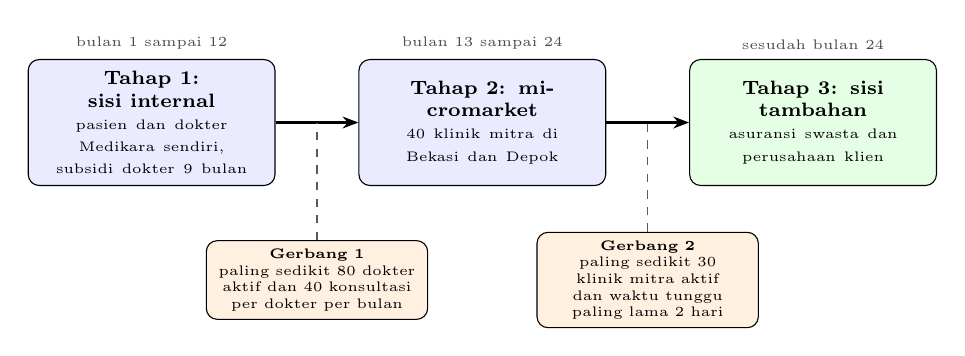
\begin{tikzpicture}[
  font=\scriptsize,
  tahap/.style={draw, rounded corners, minimum height=1.6cm, text width=2.9cm,
                align=center, font=\scriptsize\bfseries},
  gerbang/.style={draw, rounded corners, fill=orange!12, text width=2.6cm,
                  align=center, font=\tiny, inner sep=3pt},
  panah/.style={-{Stealth[length=2mm]}, thick},
  garis/.style={dashed, gray!70!black}
]
  \node[tahap, fill=blue!8] (satu) at (0,0)
    {Tahap 1: sisi internal\\{\tiny\mdseries pasien dan dokter Medikara sendiri,
     subsidi dokter 9 bulan}};
  \node[tahap, fill=blue!8] (dua) at (4.2,0)
    {Tahap 2: micromarket\\{\tiny\mdseries 40 klinik mitra di Bekasi dan Depok}};
  \node[tahap, fill=green!10] (tiga) at (8.4,0)
    {Tahap 3: sisi tambahan\\{\tiny\mdseries asuransi swasta dan perusahaan klien}};

  \draw[panah] (satu) -- (dua);
  \draw[panah] (dua) -- (tiga);

  \node[gerbang] (g1) at (2.1,-2.0)
    {\textbf{Gerbang 1}\\paling sedikit 80 dokter aktif dan 40 konsultasi per dokter per bulan};
  \node[gerbang] (g2) at (6.3,-2.0)
    {\textbf{Gerbang 2}\\paling sedikit 30 klinik mitra aktif dan waktu tunggu paling lama 2 hari};
  \draw[garis] (g1.north) -- (2.1,0);
  \draw[garis] (g2.north) -- (6.3,0);

  \node[font=\tiny, text=gray!60!black, anchor=south] at (satu.north) {bulan 1 sampai 12};
  \node[font=\tiny, text=gray!60!black, anchor=south] at (dua.north) {bulan 13 sampai 24};
  \node[font=\tiny, text=gray!60!black, anchor=south] at (tiga.north) {sesudah bulan 24};
\end{tikzpicture}
}

  \vspace{4pt}
  \raggedright
  {\footnotesize \textit{Single-side}: misalkan modul gratis bagi 40 klinik mitra, 1.500 kunjungan per klinik per bulan, sehingga 60.000 kunjungan per bulan langsung tercatat.\par
  \textit{Micromarket}: misalkan 60 dokter janji temu dibagi rata ke lima kota, berarti 12 per kota. Bekasi dan Depok didahulukan berarti 30 per kota.\par}
\end{frame}

\begin{frame}{{\Large Memulai dari Sisi Internal}}
  \begin{block}{Kasus Medikara Health}
    \small
    \begin{itemize}
      \item Modal \textit{follow-the-rabbit} dan \textit{seeding}: 1,2 juta kunjungan per tahun dan ratusan dokter internal.
      \item Tahap 1, bulan 1 sampai 12: jaminan honor minimum selama sembilan bulan bagi dokter internal.
      \item Tahap 2, bulan 13 sampai 24: 40 klinik mitra di Bekasi dan Depok mendapat modul jadwal gratis.
      \item Konsekuensi pertama: direksi perlu menyetujui biaya tahun pertama tanpa pendapatan platform.
      \item Konsekuensi kedua: kota lain menunggu paling cepat sampai tahun ketiga.
    \end{itemize}
  \end{block}
\end{frame}

\section{Harga, Multi-Homing, dan Batas Platform}

\begin{frame}{\hfill}
  \centering
  \Huge{\textbf{Harga, Multi-Homing,\\dan Batas Platform}}
\end{frame}

\begin{frame}{{\Large Siapa yang Membayar}}
  \begin{itemize}
    \item Rochet dan Tirole: yang menentukan bukan hanya total harga, tetapi juga struktur harga.
    \item Parker dan Van Alstyne: menggratiskan produk bagi satu sisi dapat menguntungkan bila permintaan sisi lain naik.
    \item Eisenmann dan rekan menamai sisi subsidi (\textit{subsidy side}) dan sisi pembayar (\textit{money side}).
    \item FreePC 1999: pemasang iklan kurang tertarik, tawaran dihentikan setelah rugi 80 juta dolar Amerika Serikat.
    \item Setiap subsidi perlu ditulis bersama tujuan dan syarat berhentinya.
  \end{itemize}
  \vspace{2pt}
  {\footnotesize Analogi: pusat perbelanjaan. Pengunjung masuk tanpa membayar, penyewa toko membayar sewa.\par}
\end{frame}

\begin{frame}{{\Large Enam Faktor Penentu Sisi Subsidi}}
  \scriptsize
  \begin{tabularx}{\textwidth}{>{\raggedright\arraybackslash}p{2.8cm}
      >{\raggedright\arraybackslash}X
      >{\raggedright\arraybackslash}X}
    \hline
    \textbf{Faktor} & \textbf{Pertanyaan kunci} & \textbf{Penilaian Medikara+} \\ \hline
    Penangkapan efek lintas sisi & Dapatkah sisi yang disubsidi bertransaksi dengan sisi pembayar milik pesaing? & Ya, pasien dapat memesan dokter di aplikasi lain, sehingga subsidi mudah bocor \\ \hline
    Kepekaan terhadap harga & Sisi mana yang permintaannya paling turun bila dikenai biaya? & Pasien lebih peka \\ \hline
    Kepekaan terhadap mutu & Sisi mana yang menuntut mutu, dan sisi mana yang memasoknya? & Pasien menuntut mutu, dokter dan klinik memasoknya \\ \hline
    Biaya melayani pengguna tambahan & Apakah subsidi untuk satu pengguna tambahan hampir tanpa biaya? & Tidak; satu konsultasi gratis tetap memerlukan honor dokter \\ \hline
    Efek sisi sama & Apakah sisi itu lebih suka pesaingnya sedikit? & Klinik di satu kecamatan yang sama saling berebut pasien \\ \hline
    Nilai merek pengguna & Adakah peserta bergengsi yang menarik sisi lain? & Klinik mitra besar dan dokter spesialis yang dikenal luas \\ \hline
  \end{tabularx}
\end{frame}

\begin{frame}{{\Large Dua Opsi Struktur Harga}}
  \small Misalkan biaya bagi mitra Rp2,4 miliar per tahun. Skenario harga: 240.000 pemesanan per tahun pada 40 klinik mitra, terpisah dari angka dasar 28.000 per bulan.

  \vspace{2pt}
  \footnotesize
  \begin{tabularx}{\textwidth}{>{\raggedright\arraybackslash}p{2.6cm}
      >{\raggedright\arraybackslash}X
      >{\raggedright\arraybackslash}X}
    \hline
    \textbf{Aspek} & \textbf{Opsi pertama: pasien membayar} & \textbf{Opsi kedua: pasien gratis} \\ \hline
    Beban biaya & Pasien Rp10.000 per pemesanan & 40 klinik mitra Rp3 juta per bulan; asuransi swasta Rp10.000 per verifikasi \\ \hline
    Volume pemesanan & Misalkan 30\% kembali menelepon: turun menjadi 168.000 & Tidak tertekan; 40\%, yaitu 96.000 pemesanan, dijamin asuransi swasta \\ \hline
    Pendapatan per tahun & Rp1,68 miliar, kurang Rp720 juta dari biayanya & Rp1,44 miliar ditambah Rp960 juta, total Rp2,4 miliar \\ \hline
    Akibat lain & Klinik mitra melihat pasien berkurang, sebagian ikut pergi & Biaya tertutup tanpa menekan volume. Bab 12: Rp3 juta menjadi paket sedang \\ \hline
  \end{tabularx}
\end{frame}

\begin{frame}{{\Large Simulasi Empat Skenario Subsidi}}
  \centering
  \resizebox{!}{0.6\textheight}{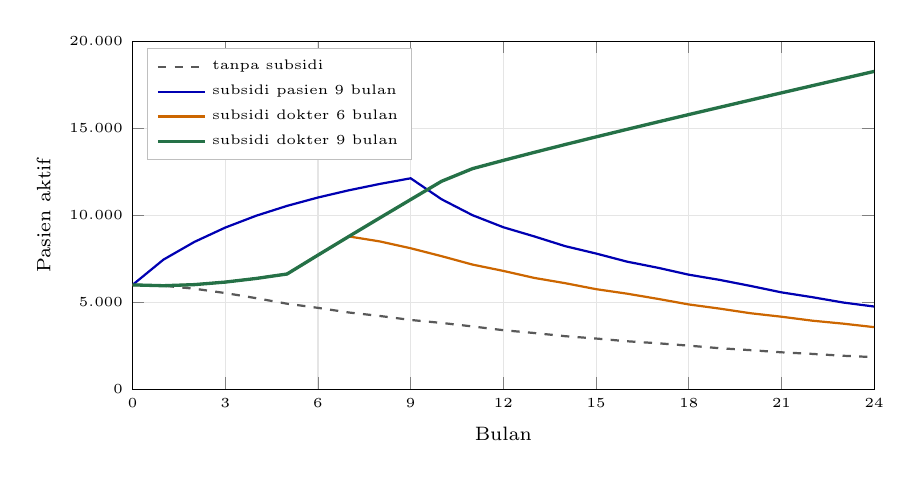
\begin{tikzpicture}[font=\scriptsize]
  \begin{axis}[
    width=11cm, height=6cm,
    xmin=0, xmax=24, ymin=0, ymax=20000,
    xtick={0,3,6,9,12,15,18,21,24},
    xlabel={Bulan}, ylabel={Pasien aktif},
    scaled y ticks=false,
    yticklabel style={/pgf/number format/.cd, 1000 sep={.}},
    tick label style={font=\tiny},
    label style={font=\scriptsize},
    legend style={font=\tiny, at={(0.02,0.98)}, anchor=north west, draw=gray!50},
    legend cell align=left,
    grid=major, grid style={gray!20},
    every axis plot/.append style={thick, mark=none}
  ]
    \addplot[gray!70!black, dashed] coordinates {
      (0,6000) (1,5952) (2,5780) (3,5531) (4,5236) (5,4918) (6,4680) (7,4413)
      (8,4214) (9,3984) (10,3813) (11,3612) (12,3395) (13,3233) (14,3051)
      (15,2916) (16,2760) (17,2644) (18,2507) (19,2359) (20,2248) (21,2124)
      (22,2032) (23,1925) (24,1846)};
    \addlegendentry{tanpa subsidi}
    \addplot[blue!70!black] coordinates {
      (0,6000) (1,7452) (2,8470) (3,9295) (4,9975) (5,10542) (6,11023)
      (7,11438) (8,11803) (9,12128) (10,10923) (11,10008) (12,9313) (13,8787)
      (14,8227) (15,7803) (16,7337) (17,6985) (18,6586) (19,6287) (20,5940)
      (21,5570) (22,5293) (23,4985) (24,4755)};
    \addlegendentry{subsidi pasien 9 bulan}
    \addplot[orange!80!black] coordinates {
      (0,6000) (1,5952) (2,6015) (3,6161) (4,6370) (5,6626) (6,7712) (7,8785)
      (8,8499) (9,8106) (10,7651) (11,7168) (12,6803) (13,6401) (14,6098)
      (15,5754) (16,5496) (17,5196) (18,4876) (19,4636) (20,4370) (21,4170)
      (22,3942) (23,3771) (24,3571)};
    \addlegendentry{subsidi dokter 6 bulan}
    \addplot[praditagreen, very thick] coordinates {
      (0,6000) (1,5952) (2,6015) (3,6161) (4,6370) (5,6626) (6,7712) (7,8785)
      (8,9849) (9,10905) (10,11956) (11,12682) (12,13157) (13,13618)
      (14,14068) (15,14508) (16,14941) (17,15368) (18,15791) (19,16209)
      (20,16625) (21,17039) (22,17451) (23,17862) (24,18272)};
    \addlegendentry{subsidi dokter 9 bulan}
  \end{axis}
\end{tikzpicture}
}

  \vspace{2pt}
  \raggedright
  {\scriptsize Awal: 6.000 pasien dan 60 dokter. Bulan 24: tanpa subsidi 1.846 pasien; subsidi pasien Rp675 juta, 4.755 pasien; subsidi dokter 6 bulan Rp376 juta, 3.571 pasien; subsidi dokter 9 bulan Rp578 juta, 18.272 pasien. Pendalaman opsional: \berkas{sources/chapter02/simulasi-dua-sisi.py}.\par}
\end{frame}

\begin{frame}{{\Large Siapa yang Menanggung Biaya Platform}}
  \begin{block}{Kasus Medikara Health}
    \small
    \begin{itemize}
      \item Pasien tidak dikenai biaya pemesanan, tetapi tetap membayar tarif konsultasi.
      \item Klinik mitra mendapat masa uji enam bulan, lalu membayar langganan bulanan.
      \item Asuransi swasta membayar per verifikasi. Perusahaan klien membayar paket per karyawan pada Tahap 3.
      \item Medikara menanggung seluruh biaya platform sekitar 18 bulan sejak peluncuran.
      \item Klinik mitra hanya mau membayar bila Medikara+ benar-benar mengirim pasien, sehingga pemesanan per klinik dipantau sejak bulan pertama Tahap 2.
    \end{itemize}
  \end{block}
\end{frame}

\begin{frame}{{\Large Multi-Homing dan Disintermediasi}}
  \begin{itemize}
    \item \textit{Multi-homing}: berafiliasi dengan lebih dari satu platform sejenis pada saat yang sama.
    \item Biaya berpindah: riwayat yang tertinggal dan kontrak yang harus diputus.
    \item Armstrong: platform memperebutkan sisi \textit{single-homing}, lalu menarik harga tinggi dari sisi \textit{multi-homing}.
    \item Misalkan 62\% pengguna Medikara+ juga memasang aplikasi kesehatan lain.
    \item Disintermediasi: misalkan dari 1.000 pasien yang bertemu dokter klinik mitra lewat aplikasi, 650 (65\%) lalu menelepon klinik langsung.
  \end{itemize}
  \vspace{2pt}
  {\footnotesize Penangkalnya nilai yang hanya ada di platform, misalnya rekam medis lintas fasilitas dan resep elektronik.\par}
\end{frame}

\begin{frame}{{\Large Diagram Konsep Bab 2}}
  \centering
  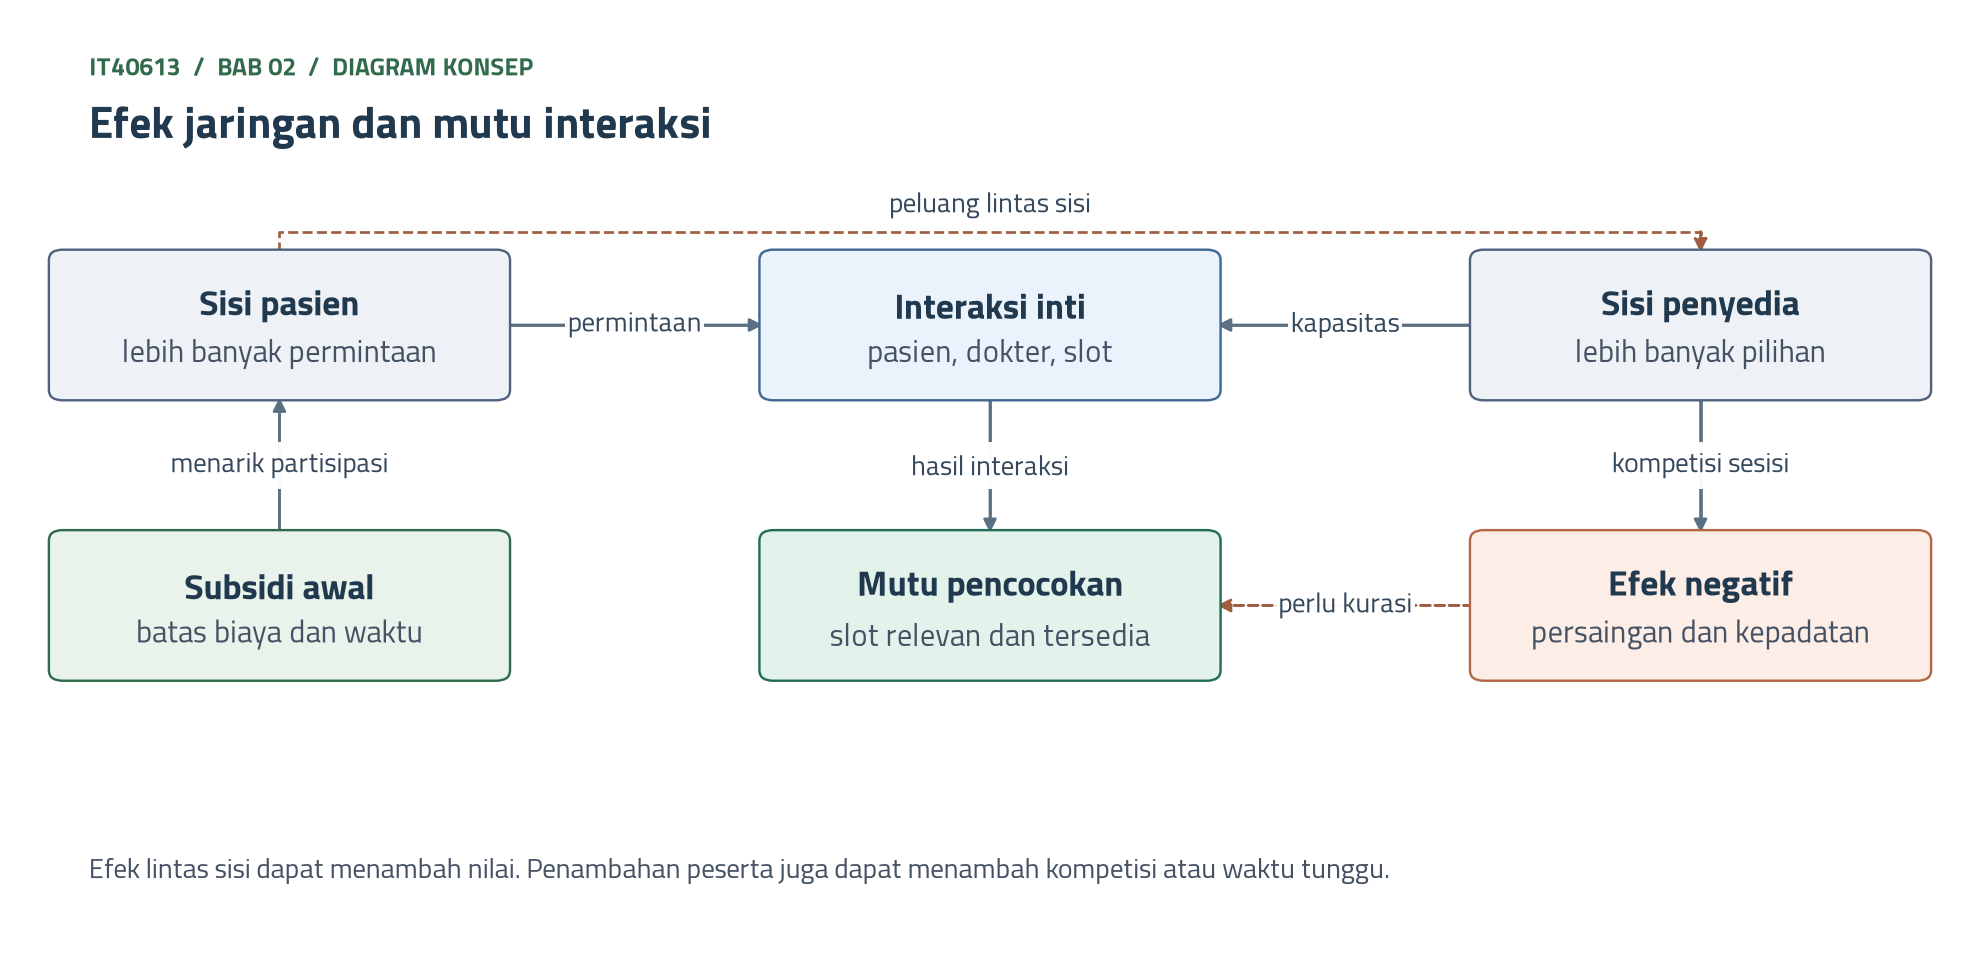
\includegraphics[width=0.96\textwidth,height=0.77\textheight,keepaspectratio]{../../figures/ch02-diagram-konsep.png}
\end{frame}

\begin{frame}{{\Large Kondisi yang Melemahkan Model Platform}}
  \scriptsize
  \begin{tabularx}{\textwidth}{>{\raggedright\arraybackslash}p{3.0cm}
      >{\raggedright\arraybackslash}X
      >{\raggedright\arraybackslash}X}
    \hline
    \textbf{Kondisi} & \textbf{Mengapa melemahkan} & \textbf{Keadaan Medikara} \\ \hline
    Interaksi jarang & Pengguna tidak kembali, efek jaringan tidak sempat terbentuk & Tindakan besar seperti operasi jantung jarang berulang \\ \hline
    \textit{Multi-homing} murah & Pengguna mudah pergi; harga sulit dinaikkan & Pasien memasang beberapa aplikasi tanpa biaya \\ \hline
    Produsen langka & Sisi produsen tidak dapat diperbanyak cepat & Dokter spesialis terbatas dan banyak yang berpraktik di beberapa tempat \\ \hline
    Tanggung jawab melekat pada penyedia & Platform harus mengkurasi ketat, sehingga makin mirip \textit{pipeline} & Fasilitas kesehatan bertanggung jawab atas layanan, termasuk telemedisin menurut UU 17/2023 \\ \hline
    Data sensitif & Data tidak bebas mengalir antarsisi & Data kesehatan adalah data pribadi spesifik menurut UU PDP \\ \hline
    Satu pembayar dominan & Struktur harga tidak bebas diatur & Tarif program Jaminan Kesehatan Nasional ditetapkan di luar Medikara \\ \hline
  \end{tabularx}
\end{frame}

\begin{frame}{{\Large Platform untuk Sebagian Layanan}}
  \begin{block}{Kasus Medikara Health}
    \small
    \begin{itemize}
      \item Pasien melakukan \textit{multi-homing} dengan murah. Misalkan 55\% dokter spesialis juga berpraktik di rumah sakit lain.
      \item Aset yang sulit ditiru: rekam medis lintas fasilitas sesuai strategi ``Satu Pasien, Satu Rekam Medis''.
      \item Bila hanya dapat diakses lengkap lewat Medikara+, biaya berpindah pasien naik tanpa penguncian yang tidak adil.
      \item Model hibrida: platform untuk janji temu rawat jalan, telekonsultasi, dan layanan kesehatan karyawan di Bekasi dan Depok.
      \item Rawat inap dan tindakan besar tetap dijalankan sebagai \textit{pipeline}.
    \end{itemize}
  \end{block}
\end{frame}

\section{Aktivitas, Ringkasan, dan Latihan}

\begin{frame}{\hfill}
  \centering
  \Huge{\textbf{Aktivitas, Ringkasan,\\dan Latihan}}
\end{frame}

\begin{frame}{{\Large Aktivitas: Kanvas dan Peta Efek Jaringan}}
  \begin{itemize}
    \item Tujuan: menguji apakah organisasi capstone punya dasar untuk menjadi platform.
    \item Peran: pemimpin analisis sisi pasar, penelaah data dan sistem, penelaah regulasi, penyunting.
    \item Langkah: interaksi inti satu kalimat, kanvas platform, asal unit nilai, peta efek jaringan, daftar periksa kecocokan, catatan subsidi.
    \item Luaran masuk ke tonggak C1 Konteks dan Strategi.
    \item Penilaian: lima kriteria, masing-masing 20\%.
  \end{itemize}
  \vspace{2pt}
  {\footnotesize Data organisasi nyata dipakai seizin organisasi dan dianonimkan. Berkas: \berkas{sources/chapter02/}.\par}
\end{frame}

\begin{frame}{{\Large Ringkasan}}
  \vspace{6pt}
  \begin{itemize}
    \item Interaksi langsung dan afiliasi membedakan platform dari pengecer dan dari \textit{pipeline}.
    \item Interaksi inti Medikara+ adalah janji temu: 336.000 per tahun, jauh di atas telekonsultasi yang 21.600.
    \item Efek jaringan dibedakan menurut arah dan tanda. Janji temu bersifat lokal: empat dokter anak di Bogor.
    \item Subsidi dokter sembilan bulan senilai Rp578 juta melewati titik kritis, subsidi pasien senilai Rp675 juta tidak.
    \item Menjadi platform merupakan keputusan model bisnis, bukan keputusan teknologi.
  \end{itemize}
\end{frame}

\begin{frame}{{\Large Latihan}}
  \vspace{6pt}
  \begin{itemize}
    \item Latihan 1, Sisi yang Disubsidi pada Platform Telekonsultasi: sisi subsidi, bentuk subsidi, dan syarat berhentinya.
    \item Latihan 2, Efek Jaringan Negatif dan Mekanisme Penekannya: indikator terukur, efek samping, target tiga bulan.
    \item Latihan 3, Kecocokan Jaringan Rumah Sakit Menjadi Platform: platform penuh, hibrida, atau tetap \textit{pipeline}.
  \end{itemize}
  \vspace{6pt}
  {\small Tidak membutuhkan kemampuan memprogram. Yang dinilai adalah penalaran dan perbandingannya. Berkas: \berkas{sources/chapter02/}.\par}
\end{frame}

\end{document}
